\documentclass[12pt,a4paper]{article}

\usepackage{fontspec}
\usepackage{polyglossia}
\usepackage[left=3cm,top=2cm,right=1cm,bottom=2cm,nohead]{geometry}
\usepackage{setspace}
\usepackage{listings}
\usepackage{alltt}
\usepackage{graphicx}
\usepackage{color}
\usepackage{float}
\usepackage{courier}
\usepackage{bold-extra}
\usepackage{fix-cm}
\usepackage{alltt}
\usepackage{indentfirst}
\usepackage{amsmath, amsthm, amssymb}
\usepackage{url}

\defaultfontfeatures{Mapping=tex-text}

\setmainfont
    [ Path           = fonts/ ,
      UprightFont    = *-Regular,
      BoldFont       = *-Bold ,
      ItalicFont     = *-Italic ,
      BoldItalicFont = *-BoldItalic]
    {LiberationSerif}
\setsansfont
    [ Path           = fonts/ ,
      UprightFont    = *-Regular,
      BoldFont       = *-Bold ,
      ItalicFont     = *-Italic ,
      BoldItalicFont = *-BoldItalic]
    {LiberationSans}
\setmonofont
    [ Path           = fonts/ ,
      UprightFont    = *-Regular,
      BoldFont       = *-Bold ,
      ItalicFont     = *-Italic ,
      BoldItalicFont = *-BoldItalic]
    {LiberationMono}

\setmainlanguage{ukrainian}
\setotherlanguage{english}

\graphicspath{{./images/}}

\setstretch{1.1}

\definecolor{javared}{rgb}{0.6,0,0}
\lstset{
  basicstyle=\footnotesize\ttfamily,
  tabsize=3,
  showspaces=false,
  stringstyle=\color{javared},
  showstringspaces=false,
  xleftmargin=.6cm,
  breaklines=true
}

\begin{document}
\pretolerance=-1
\tolerance=2300

\pagenumbering{arabic}
\pagestyle{empty}
\setlength{\parindent}{1.5cm}
\fontsize{14pt}{6mm}\selectfont

\begin{flushright}
  {\bfseries\small Форма № Н-9.02}
\end{flushright}

\begin{center}
  \begin{spacing}{2}
    \uppercase{
      Львівський національний університет імені Івана Франка

      Факультет прикладної математики та інформатики

      Кафедра програмування
    }
  \end{spacing}

  \vspace{6cm}


    {\bfseries\Large Магістерська робота}

    {\small (освітньо--кваліфікаційний рівень магістр)}

    \bigskip

    на тему: {\bfseries\large „Архітектурні особливості проекту створення електронної лабораторії BUMMEL“}

\end{center}

\vspace{2cm}

\begin{small}
\begin{flushleft}\leftskip8.5cm
  Виконав студент 5 курсу, групи ПМІ-51м спеціальності 8.04030201 Інформатика\\
  Михалевич І.А.\linebreak

  Керівник: доц. Рикалюк Р.Є.\linebreak

  Рецензент: \underline{\hspace{3cm}}

\end{flushleft}
\end{small}

\vspace{5cm}

\begin{center}
  Львів - 2013 року
\end{center}

\clearpage



\setstretch{1.5}
\fontsize{14pt}{6mm}\selectfont

\tableofcontents
\clearpage
\setcounter{page}{6}
\pagestyle{plain}
\section{Вступ}

Електронна лабораторія BUMMEL - це програма для моделювання логічних схем. Розробка її почалась два роки тому (2011 рік) як груповий курсовий проект. Метою даного проекту є вивчення сучасних технологій розробки програмного забезпечення та створення навчальної програми, яка може бути використана в курсі „Архітектура ЕОМ“ і буде зручнішою і коректнішою в роботі ніж ПЗ, яке використовується на даний момент.

Крім того, програма розробляється як вільний продукт \cite{thesis-foss2013} і будь-хто може долучитись до цього процесу.

Перед початком розробки було обрано, обдумано і складено архітектуру програми та алгоритм моделювання об’єктів дослідження.

За час розробки програми змінювалось практично все. Було опробувано різні підходи до організації робочого потоку \cite{thesis-MPoAMaCS} та вибрано найбільш зручні. Також з плином еволюції програми змінювались і технології з допомогою яких реалізовувався той чи інший функціонал (наприклад, SVG графіка та інструменти побудови виконавчого коду). При переході до версії 0.2 було виправлено та вдосконалено моделювання схем. Елементна база не стояла на місці і теж розширилась -- починалось все з базових елементів логіки, а зараз вже маємо елементи з пам’яттю.

Крім самого проекту змінилась, а точніше збільшилась і група людей, що над ним працює. Власне, нові люди допомагали з розширенням функціоналу та опробуванням нових технологій.
% \cite{на дипломні Романа і Юрка}

Як видно з короткого опису, BUMMEL - живий проект, який видозмінюється з усіх сторін. Але, якщо дивитись уважно, то видно, що змінювалось практично все, крім архітектури програми. Як на самому початку було обрано базувати програму на NetBeans Platform, а архітектурно на MVC, де, в силу архітектури основи, другий компонент абревіатури - V - View (NB Visual Library) також структурно являє собою MVC патерн. Тобто BUMMEL -- MMVCC NetBeans Platform програма.

Такий довгий період без втручань до цієї частини електронної лабораторії вказує на одне з двох: або архітектура була дуже добре складена і не потребує втручань, або, навпаки, вона дуже складна і всі бояться її модифікувати „раз і так працює“.

Насправді ситуація що склалась на сьогодні поєднує ці два варіанти. Ідейно архітектура підібрана добре, але в силу величини і, можна сказати, складності мови Java та каркасу NetBeans Platform, на практиці не доведена до бажаного стану. Декількома надлишковими зв’язками порушено структуру M(V=MVC)C. До цього також привів початковий задум - зробити найнижчу логіку програми універсальною, для можливості моделювати не лише логічні схеми, а й багато інших процесів, що можна відобразити через мережі, дерева та ін.

До архітектурної проблеми додається ще функціонально-архітектурна проблема. Як виявилось, з наявним методом моделювання ми не можемо просунутись далі ніж прості схеми з елементами пам’яті. Наприклад, вже циклічні схеми з тригерами можуть дати некоректні результати.

Для того щоб програма могла і далі розвиватись в своєму основному напрямку, а не по супутніх та додаткових гілках, потрібно викристалізувати архітектуру програми та скласти чи підібрати і адаптувати алгоритм моделювання схем. Крім того, так як програма являється і дослідницькою роботою, то потрібно створити інструменти які б спрощували, власне, дослідження тих чи інших алгоритмів та підходів в даній ситуації (для поставлених цілей і з утвореними задумами).

Це все дасть можливість:
\begin{itemize}
  \item швидше орієнтуватись в програмі та обирати область для праці (внаслідок прозорості та доступності архітектури)
  \item збільшити продуктивність команди розробників (внаслідок ширшого спектру можливостей для розвитку)
  \item в разі успіху з укладанням алгоритму моделювання логічних елементів та схем, впровадити програму в університетський навчальний курс
  \item використовувати програму як бібліотечну основу для інших задач та моделювання інших процесів
  \item спростити та гармонізувати процес розростання команди розробників, яка зростала протягом минулих років кожного року
\end{itemize}

Дана проблема, являє собою, так зване, вузьке місце, в графі розвитку програми.

Мета даної магістерської роботи - дослідити наявну архітектуру програми та метод моделювання, надати інструменти для подальших досліджень та експериментів з ними, вдосконалити архітектуру програми - виправити описану вище проблему. Також, у випадку успіху, зробити продукт який буде прийнятним для впровадження в навчальний курс „Архітектури ЕОМ“.

\clearpage

\section{Постановка задачі}

В становищі, яке склалось на даний момент в ході розробки програми для моделювання логічних схем - електронної лабораторії BUMMEL, з точки зору програмної інженерії та моделювання логічних схем виникло декілька проблем, які утворюють, так зване, вузьке місце в графі розвитку програми. Тобто, іншими словами, без вирішення їх, подальший розвиток продукту є дуже важким або обмеженим до певного рівня.

BUMMEL розроблялась і розробляється як M(V=MVC)C програма з основою на каркасі NetBeans Platform. Головні проблеми які виникли це:
\begin{enumerate}
  \item Порушення архітектури M(V=MVC)C.
  \item Недосконалість алгоритму моделювання логічних схем - некоректне моделювання циклічних схем з елементами пам’яті.
  \item Відсутність інструментів для проведення досліджень в реальному часі роботи програми.
\end{enumerate}

Наведені пункти породжують інші, менш важливі, але більш видимі проблеми. Наприклад, внаслідок порушення архітектури, розробка засобів взаємодії користувача з елементами досліджень є складною і призводить до погіршення якості коду та швидкості його сприйняття.

Тому першочерговою задачею в ході розробки BUMMEL є виправлення наведених вище недоліків. Цю задачу можна поділити на наступні завдання. Першим і найголовнішим завданням є дослідження та опис наявної ситуації, щоб можна було чітко вказати місця проблем і способи їх вирішення. Наступним завданням є більш глибоке вивчення предметної області (моделювання логічних елементів) задля розробки коректного алгоритму. В ході розробки алгоритму потрібним буде проведення дослідження різних вже відомих і добре перевірених підходів та апробації в даній програмі. Для підвищення ефективності цих процесів добре було б розробити певні інструменти підтримки, наприклад для порівняльного аналізу в реальному часі. Ще одним завданням є розкриття прихованого функціоналу програми і наближення його до користувача чи дослідника, шляхом розробки елементів користувацького інтерфейсу для взаємодії зі схемою, як це прийнято бачити в сучасних програмах.

Тобто, як видно, задачу можна поділити на дві області:
\begin{itemize}
  \item архітектура програми
  \item архітектура моделювання
\end{itemize}
в межах яких проводилась дана магістерська робота.

\clearpage

\section{Моделювання цифрових пристроїв}

При автоматизації проектування і діагностування цифрових пристроїв (ЦП) широке застосування знаходять системи моделювання. Для представлення пристроїв вони вимагають відповідних математичних моделей. При проектуванні ЦП слід розрізняти моделі пристроїв та їх специфікації. Специфікації описують пристрій в термінах одержуваних результатів проектування, таких як схеми, \emph{тимчасові діаграми} і т.п. Моделі використовуються в процедурах проектування пристроїв при моделюванні в даній області (\emph{domain}), на даному рівні подання для перевірки відповідності вказаним специфікаціям. Вони також застосовуються для встановлення відповідності між різними рівнями і областями проектування.

\subsection{Області та рівні проектування}

Залежно від поглядів на природу ЦП і його організацію, прийнято розглядати три області подання: фізична, структурна і поведінкова, які показані на рис.~\ref{abstrLvlDiag}. Для кожної з цих областей розрізняють різні рівні: схемний, логічний, мов реєстрових передач (МРП) і системний. При цьому в поведінковій області дається функціональне уявлення ЦП, у структурній області описуються блоки архітектури ЦП, фізична область відображає реальний кристал (\emph{chip}). Наприклад, для логічного рівня ці три області показані на рис.~\ref{logicLvl}.

\begin{figure}[h]
  \centering
    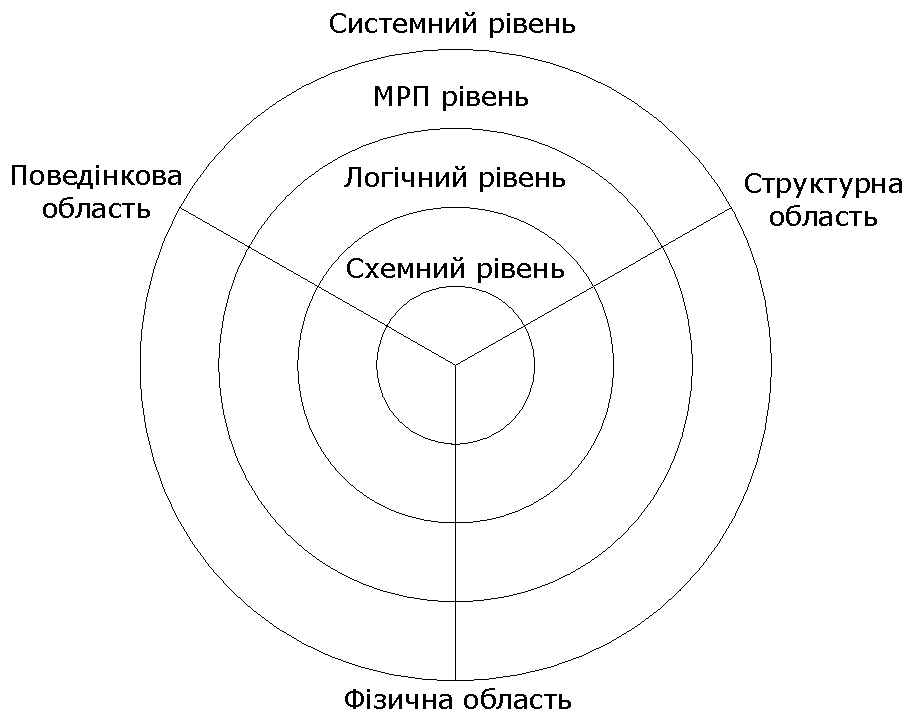
\includegraphics[width=0.5\textwidth]{Gajsky-and-Kuhn-diagram}
  \caption{Діаграма рівнів абстракції (Гайського-Кана)\label{abstrLvlDiag}}
\end{figure}

\begin{figure}[h]
  \centering
    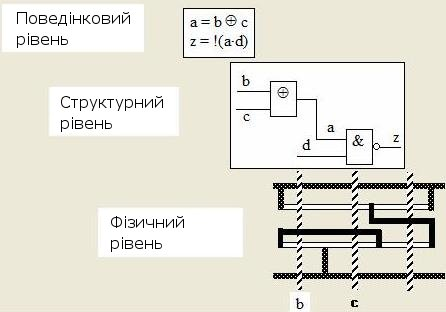
\includegraphics[width=0.5\textwidth]{logic-level-presentation-domains.jpg}
  \caption{Області представлення схеми на логічному рівні\label{logicLvl}}
\end{figure}

\subsection{Склад і призначення програм логічного моделювання}

Логічне моделювання являє собою процедуру перевірки функціонування логічної схеми за допомогою комп'ютера. Його основна мета полягає в тому, щоб перевірити функцію проектованої логічної схеми без її фізичної реалізації, оскільки після виготовлення схеми внесення змін до неї за сучасної технології зробити нелегко і недешево. Верифікація виконується шляхом порівняння результатів моделювання, отриманих для проектованого ЦП, зі специфікацією. При цьому перевіряються як логічні функції, так і тимчасові співвідношення.

Логічне моделювання включає в себе побудову математичної моделі ЦП - системи співвідношень, що описує поведінку досліджуваного пристрою із заданою точністю, і подальший аналіз поведінки цієї моделі на заданій послідовності вхідних впливів. При вирішенні завдань аналізу і діагностування ЦП зазвичай використовується структурна математична модель об'єкта, що відображає сукупність компонентів об'єкта, зв'язки між компонентами і зв'язок об'єкта із зовнішнім середовищем. Для виконання логічного моделювання необхідні наступні компоненти, представлені на рис.~\ref{logicModStruct}.
\begin{itemize}
  \item модель ЦП;
  \item вхідні впливи;
  \item бібліотека логічних елементів;
  \item результати моделювання.
\end{itemize}
Тут зовнішній опис схеми (графічний або текстовий на спеціалізованій мові) транслюється у внутрішнє представлення моделі ЦП, яке безпосередньо використовується в процесі моделювання. Вхідні дії також можуть бути описані графічно за допомогою тимчасових діаграм або текстом на спеціалізованій мові. Найважливішою компонентою є бібліотека моделей логічних елементів, склад якої багато в чому визначає можливості системи моделювання. Результатом є зміна сигналів у часі для зовнішніх і внутрішніх змінних моделі у вигляді таблиць або тимчасових діаграм, які записуються на диск.

\begin{figure}[h]
  \centering
    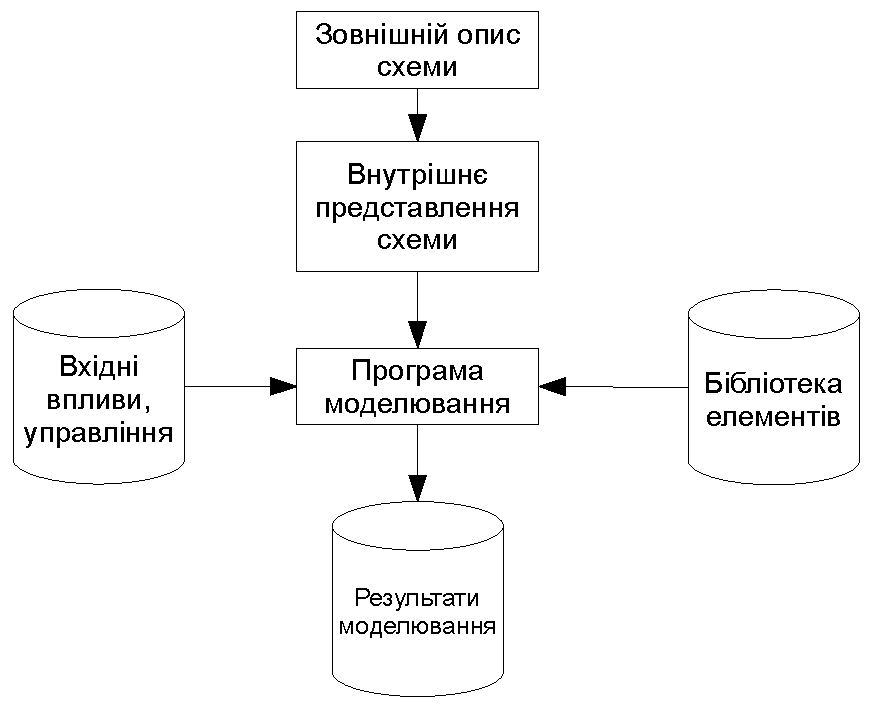
\includegraphics[width=0.75\textwidth]{logic-modelling-system-structure}
  \caption{Структура системи логічного моделювання\label{logicModStruct}}
\end{figure}

Логічне моделювання є найважливішою компонентою САПР цифрових систем. За допомогою логічного моделювання в системах автоматизованого проектування та діагностування ЦП досліджуються наступні проблеми~\cite{bib-logModNTest}:
\begin{itemize}
  \item перевірка правильності логічного функціонування ЦП;
  \item перевірка функціонування ланцюгів установки ЦП;
  \item перевірка часових характеристик ЦП;
  \item аналіз змагань сигналів;
  \item визначення повноти тесту та списку неперевірених несправностей;
  \item визначення діагностичних властивостей тестів;
  \item отримання діагностичної інформації для локалізації несправностей ЦП.
\end{itemize}

При верифікації ЦП з допомогою логічного моделювання необхідно вирішити такі проблеми:
\begin{itemize}
  \item побудова необхідних вхідних впливів (генерація тестів);
  \item визначення коректності отриманих результатів;
  \item визначення якості використовуваних вхідних впливів (наприклад, повнота перевіряючих тестів тощо).
\end{itemize}

Основним математичним апаратом, вживаним в дослідженні цифрових логічних схем, є теорія булевих функцій. При цьому функціонування ЦП моделюється в двійковому алфавіті, що досить точно відображає їх поведінку в статиці для сталих значень сигналів. Однак такі моделі не враховують перехідні процеси, що виникають при зміні значень вхідних сигналів і зумовлені часовими характеристиками елементів. Тому при дослідженні перехідних процесів набули поширення багатозначні алфавіти, які дозволяють вирішувати ці завдання з відомим ступенем адекватності логічними засобами без явного завдання затримок елементів. Зазначимо, що в разі аналізу перехідних процесів ми маємо ЦП в два різні (попередній і справжній) моменти часу і безліч ліній, на яких значення сигналів в ці моменти різні (або можуть бути різні) внаслідок зміни деяких вхідних сигналів. З іншого боку, при синтезі тестів ми маємо один ЦП в двох різних технічних станах (справний і несправний) і безліч ліній схеми, на яких значення сигналів у цих станах різні (або можуть бути різні) внаслідок наявності в деяких елементах несправностей. В обох випадках ми досліджуємо логічну залежність в ЦП: при моделюванні внаслідок зміни вхідних сигналів, при генерації тестів - ефект впливу несправностей. Тому, в силу однакової математичної природи при побудові тестів також широко використовуються багатозначні алфавіти. В обох випадках аналіз двох ЦП в двійковому (іноді трійковому) алфавіті замінюється аналізом одного пристрою в багатозначному алфавіті.

\subsection{Загальні принципи логічного моделювання}

Вихідною інформацією для програм логічного моделювання є опис схеми ЦП у вигляді мережі, вершинами якої є логічні елементи, входи і виходи. Практично кожна система моделювання має свої мовні засоби для опису схеми ЦП і вхідних впливів (тестів).

Далі опис схеми транслюється в деяке внутрішнє машинне представлення, яке дозволяє ефективно виконувати власне процес моделювання. Існує два основних типи машинних моделей схеми: таблична і програмна. Відповідно до цього використовуються два методи моделювання: інтерпретативний і компілятивний. Інтерпретативне моделювання використовує модель схеми у вигляді ряду таблиць, пов'язаних системою посилань, є більш універсальним і дозволяє проводити більш точний часовий аналіз. Компілятивний метод моделювання використовує готову скомпільовану машинну програму і тому є більш швидкодіючим за рахунок скорочення операцій пошуку адрес потрібних значень сигналів і викликів підпрограм, які становлять істотну частину в інтерпретативній методі.

\begin{figure}[h]
  \centering
    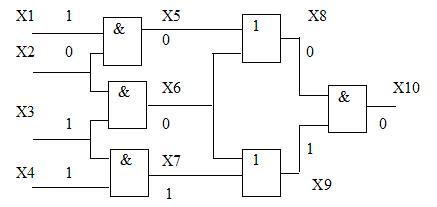
\includegraphics[width=0.5\textwidth]{03_02.jpg}
  \caption{Приклад логічного моделювання схеми\label{logicModEx}}
\end{figure}

Процес логічного моделювання складається з подачі на зовнішні входи моделі ЦП деякого вхідного впливу і послідовного від входів схеми до її виходів обчислення значень виходів логічних елементів і отримання, таким чином, вихідний реакції на заданий вхідний вплив. На рис.~\ref{logicModEx} представлений простий приклад комбінаційної схеми з результатами логічного моделювання в двійковому алфавіті для одного вхідного набору (відповідний одного моменту часу).

Цей процес може бути організований по-різному залежно від застосовуваних методів моделювання. Основними виразними рисами методів логічного моделювання є: модель сигналів, модель схеми в комп'ютері, спосіб обліку часу поширення сигналів в ЦП, управління черговістю моделювання логічних елементів. Залежно від застосовуваних моделей сигналів, методи діляться: за алфавітом - на виконавчі і багатозначні; за використовуваною моделлю схеми в комп'ютері - на інтерпретативні і компілятивні; за способом розповсюдження сигналів - на синхронні (без урахування затримок логічних елементів) і асинхронні (з урахуванням затримок); за черговістю моделювання логічних елементів - наскрізні і подієві. Класифікація методів моделювання представлена ​​на рис.~\ref{logicModMethods}.

\begin{figure}[h]
  \centering
    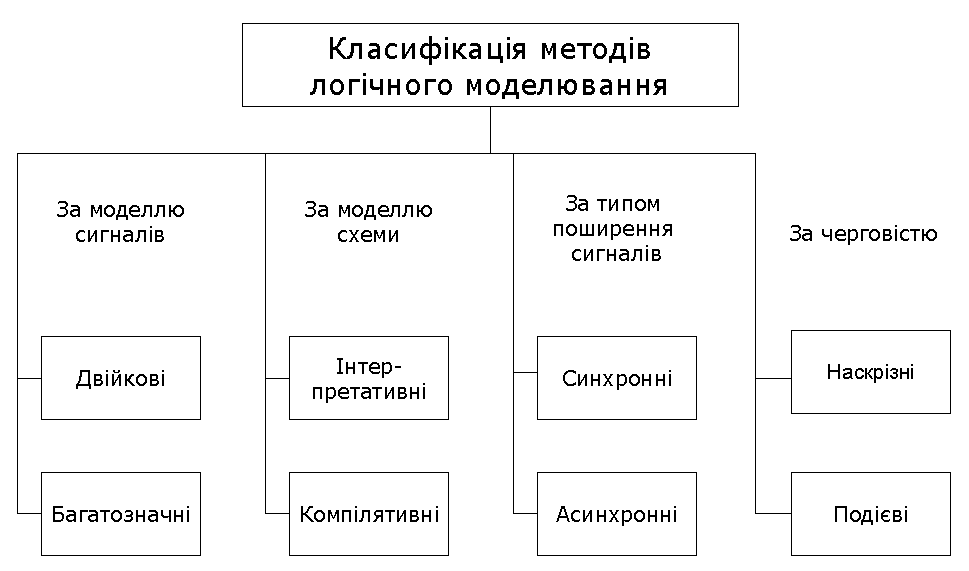
\includegraphics[width=0.8\textwidth]{logic-modelling-methods-classification}
  \caption{Методи логічного моделювання\label{logicModMethods}}
\end{figure}

Основними характеристиками алгоритмів \emph{логічного моделювання} є \emph{адекватність}, \emph{швидкодія} й \emph{обсяг} пам'яті, необхідний при реалізації. При цьому під адекватністю розуміється ступінь відповідності результатів моделювання реальній поведінці досліджуваного ЦП. Для комбінаційних ЦП всі алгоритми логічного моделювання гарантують високу адекватність сталих значень сигналів. Моделювання послідовних ЦП може давати результати різного ступеня адекватності через різні моделі затримок елементів, невизначеності початкових станів та явища змагань сигналів, що істотно ускладнює моделювання таких пристроїв.

Адекватність моделювання залежить, в основному, від використовуваної моделі ЦП, моделей логічних елементів і сигналів, способу обчислення тимчасових співвідношень між сигналами. Зазвичай підвищення ступеня адекватності пов'язане зі зниженням швидкодії і збільшенням необхідного обсягу пам'яті. Найшвидшими є алгоритми двійкового моделювання в алфавіті \{0, 1\} без урахування затримок, де реальний порядок спрацьовування елементів не береться до уваги. Обчислення затримок елементів знижує швидкодію. Аналіз перехідних процесів вимагає збільшення кількості символів алфавіту.

\clearpage

\section{Архітектура програми}

Основна структура програми являє собою три NetBeans Platform Application модулі:
\begin{enumerate}
  \item \textbf{BUMMEL-app} -- головний модуль всього проекту.
  \begin{enumerate}
    \item \textbf{ProjectModel} -- модуль, що включає в себе модель програми (частина патерну MVC).
    \item \textbf{VisualEditor} -- модуль в який входить контролер і вигляд (частини патерну MVC).
  \end{enumerate}
\end{enumerate}
Також, базовий набір елементної бази входить в модуль \textbf{LogicElements}, і являє собою зразок для написання інших модулів-пакетів елементної бази.

\begin{figure}[h]
  \centering
    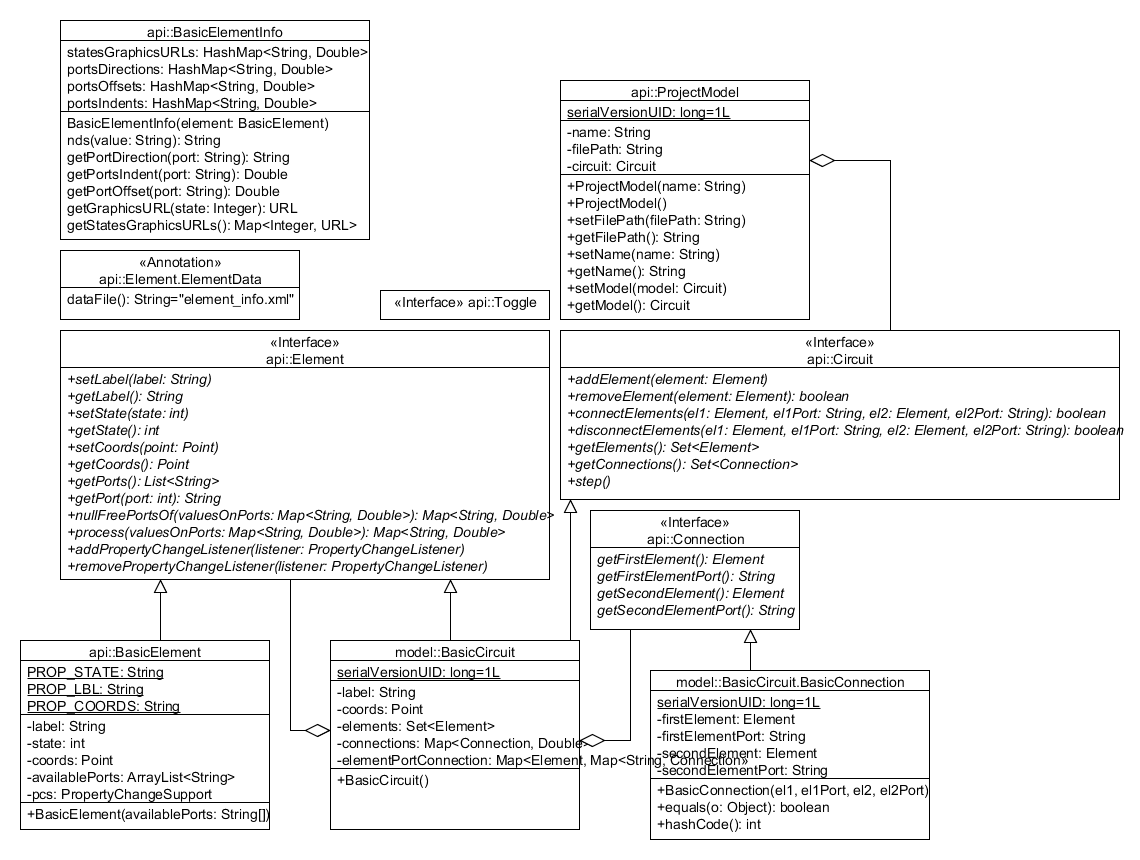
\includegraphics[width=0.95\textwidth]{class-diagram-model.png}
  \caption{Наявна структура класів Моделі BUMMEL\label{structModel}}
\end{figure}

\begin{figure}[h]
  \centering
    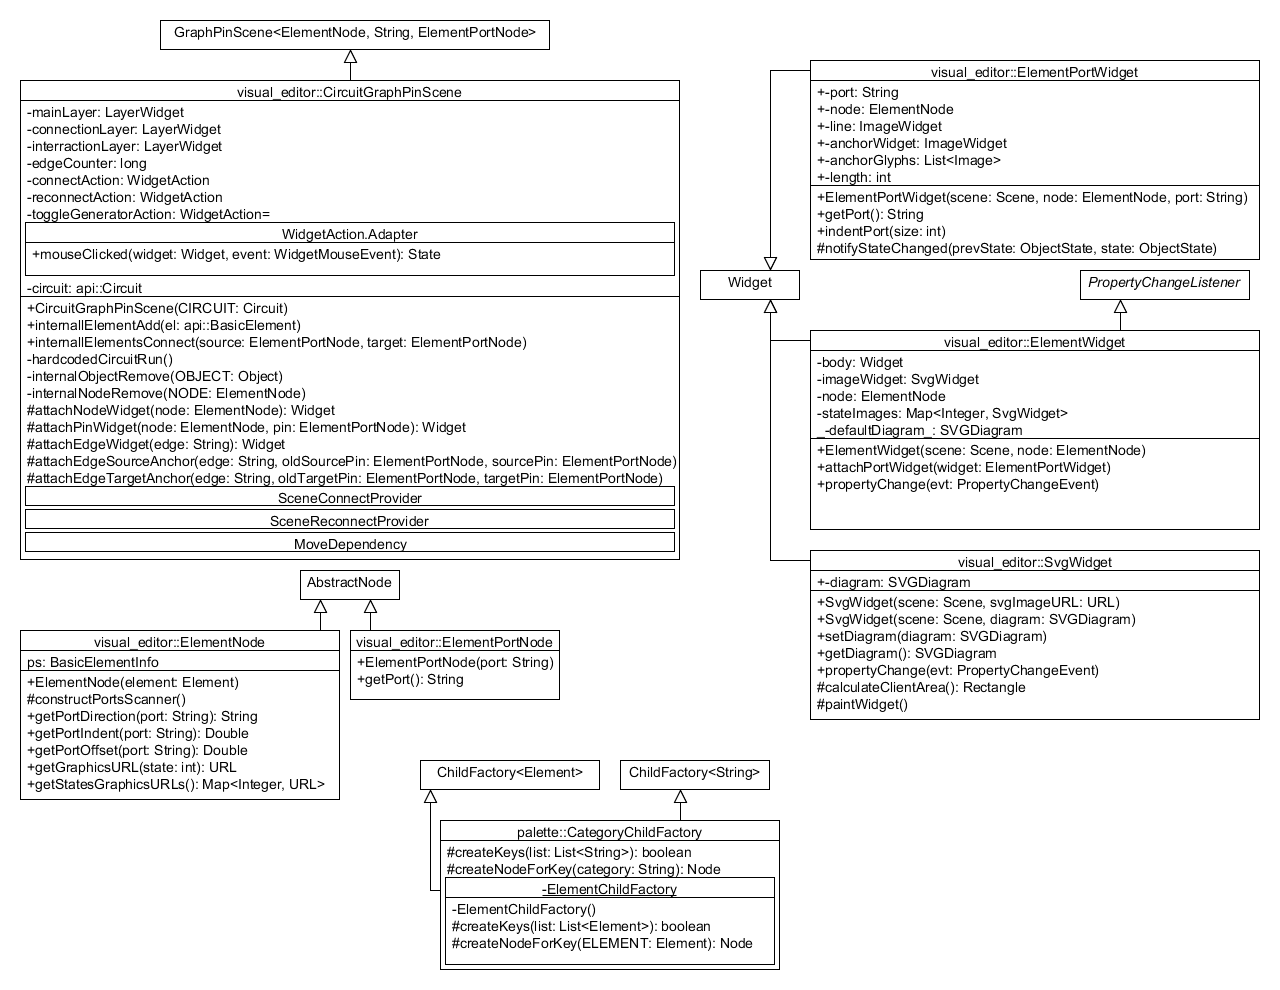
\includegraphics[width=0.95\textwidth]{class-diagram-view-NBVL.png}
  \caption{Наявна структура класів Вигляду BUMMEL\label{structView}}
\end{figure}

\begin{figure}[h]
  \centering
    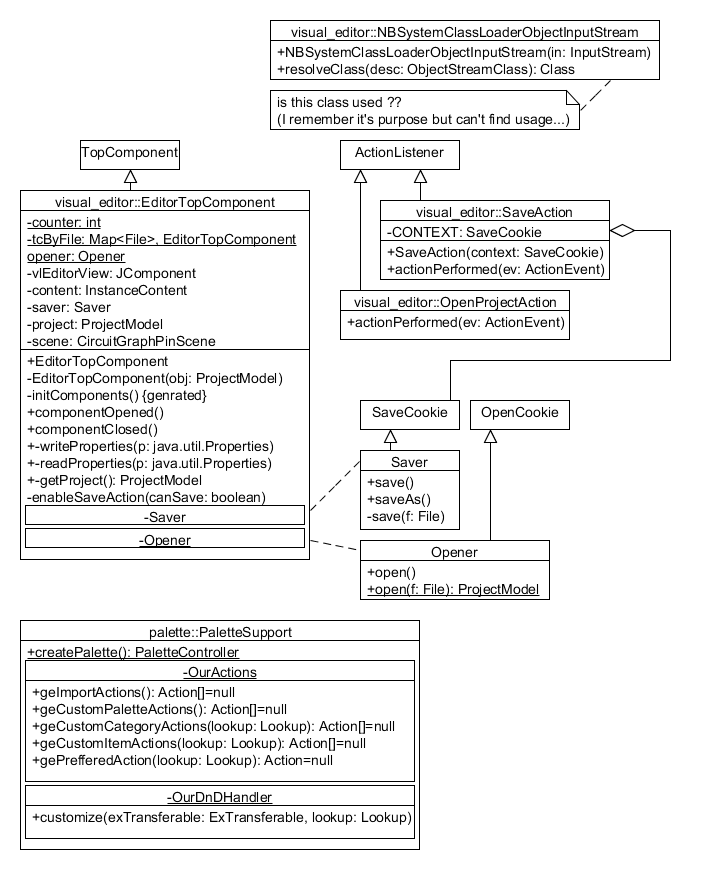
\includegraphics[width=0.75\textwidth]{class-diagram-controller.png}
  \caption{Наявна структура класів Контролера BUMMEL\label{structController}}
\end{figure}

Внаслідок проведеного аналізу архітектури програми отримано графічне представлення структури трьох головних компонентів програми:
\begin{itemize}
  \item Модель -- рис.~\ref{structModel}
  \item Вигляд -- рис.~\ref{structView}
  \item Контролер -- рис.~\ref{structController}
\end{itemize}

\clearpage

\section{Діючий алгоритм моделювання логічних схем}

\subsection{Класифікація алгоритму}

Згідно з класифікацією методів логічного моделювання, поданою в попередньому розділі, діючий алгоритм можна віднести до багатозначних інтерпретативних синхронних наскрізних алгоритмів.

Багатозначний він тому, що в програмі закладена можливість повернення довільного результату в межах \emph{double} з моделі елемента.

Хоча сама програма компілюється і елементна база також повинна бути скомпільована до початку роботи, алгоритм опрацювання схеми є інтерпретативним і використовує табличне представлення моделі.

Компілятивний підхід неможливий в даній ситуації - роботі в реальному часі користувача зі схемою. Як варіант, може бути введено попередня компіляція, але на сьогоднішній день інтерпретативний підхід працює добре, без проблем швидкодії.

Синхронність алгоритму обумовлена закладеним розробниками в основу програми принципом стабільності опрацювання схем. Так як асинхронність базується на відносних часових мірках, яку потрібно або синхронізовувати в певні моменти для подачі коректних результатів або вони будуть давати короткоімпульсні збої, які у випадку накопичення приводять до хибних результатів. Тому врахування затримок було задумано як натуральний процес дії моделей самих елементів.

В силу принципу універсальності моделі елемента (вхідні та вихідні порти елементів не розрізняються), алгоритм є наскрізним і обчислює всі елементи незалежно в декілька проходів через всю схему для отримання кінцевого результату. Кількість проходів рівна кількості елементів присутніх в схемі, це обумовлено тим, що за один прохід сигнал поширюється лише на один крок, а для поширення його по всій схемі - потрібно „прогнати“ його від початку до кінця. Причому, сам алгоритм не знає де початок, а де кінець. Це, в свою чергу, знову обумовлено принципом універсальності найнижчого рівня Моделі.

\subsection{Опис алгоритму}

Клас схеми - \lstinline$model::BasicCircuit$ - містить елементи та опрацьовує їх.
Поля класу причетні до моделювання роботи схеми:
\begin{itemize}
  \item \lstinline$elements: Set<Element>$ - контейнер, що зберігає елементи схеми
  \item \lstinline$connections: Map<Connection, Double>$ - мапа, яка зберігає значення на зв’язках.
  \item \lstinline$elementPortConnection: Map<Element, Map<String, Connection>>$ - мапа, яка портам елементів ставить у відповідність зв’язки, тобто який елемент яким портом підключений до якого зв’язка.
\end{itemize}

\textbf{„Крок“ схеми (\lstinline$BasicCircuit$):}
\begin{enumerate}
  \item Значення із зв’язків (\lstinline$BasicConnection$) перенести на порти елементів (\lstinline$BasicElement$)
  \item Опрацювати кожен елемент (лише ті що мають хоча б одне підключення) - метод \lstinline$process$, який отримує та повертає значення на портах і результати записати на зв’язки. Кожен зв’язок буде мати два значення - з портів до яких підключений.
  \item Остаточне значення на зв’язках обрахувати як середнє арифметичне значень на підключених портах.
\end{enumerate}

Дана реалізація не враховує затримок елементів явно. Затримки можуть бути реалізовані як внутрішня логіка елементів, наприклад проводити обрахунок лише через певну кількість звертань (до методу \lstinline$process$), при цьому маючи власний внутрішній лічильник.

Проблема з синхронізацією при введенні затримок - „яким чином одну ітерацію вважати як один такт або як поширювати сигнал без багаторазового обрахунку схеми“.

\clearpage

\section{Розробка нового алгоритму моделювання логічних схем}

\subsection{Подієве моделювання}

У багатьох випадках алгоритм моделювання можна представити таким чином. Після подачі вхідного впливу на модель ЦП по черзі обчислюються значення на виходах всіх елементів за значеннями на їх входах. Така процедура називається ітерацією. В результаті обчислень значення деяких сигналів можуть змінитися. У цьому випадку необхідно виконати другу ітерацію (тобто обчислити значення на виходах всіх елементів за новими значеннями на їх входах), потім третю ітерацію і так далі до тих пір, поки всі сигнали не приймуть сталих значень. У цьому випадку процес моделювання (на одному вхідному наборі) збігається природним чином. Можливий і інший результат моделювання - значення сигналів на деяких лініях періодично змінюються. У цьому випадку говорять, що моделювання не сходиться через генерації моделі ЦП. Така ситуація може бути, наприклад, в ЦП, що містить контур зворотного зв'язку з непарним числом інверсій.

Тому для збіжності процесу необхідно мати критерій закінчення моделювання. Зазвичай задають два критерії: збіг результатів моделювання на сусідніх ітераціях або досягнення деякого граничного числа ітерацій.

\small\begin{verbatim}
Подієве інтерпретативне моделювання(схема, вхідні впливи)
{
  Зчитування опису схеми;
  Зчитування вхідних впливів;
  FOR для кожного вхідного набору, який моделюється
  {
    Обробка нового вхідного набору;
    Формування нових подій, пов’язаних із зміненими входами;
    Постановка елементів, які мають події на входах,
      в чергу майбутніх подій;
    WHILE є елементи в черзі подій
    {
      Моделювання наступного елемента з черги;
      IF значення виходів елемента змінилось
      THEN Постановка всіх підключених (до виходів) елементів
        в чергу майбутніх подій відповідно
        до величини затримки елемента, що моделюється;
    }
  }
}
\end{verbatim}\normalsize

Залежно від черговості обробки логічних елементів розрізняють наскрізні і подієві методи логічного моделювання. При наскрізному методі на кожній ітерації кожен логічний елемент моделюється заново незалежно від того, відбулися зміни сигналів на його входах чи ні. У подієвому методі логічний елемент моделюється тільки в тому випадку, якщо на його входах відбулася подія - змінилося значення сигналу хоча б на одному з його входів. Для елементів пам'яті подією є також зміна його стану (зміна змінної внутрішнього стану). Зазвичай в процесі моделювання на кожній ітерації активні (мають зміни на входах) тільки кілька відсотків елементів (3-5\%), тому подієвий метод набагато швидший наскрізного.

Слід зазначити, що події відбуваються у визначені моменти часу, тому необхідний механізм моделювання тимчасової черговості подій. У наведеному вище лістингу "Подієве моделювання" представлений укрупнений алгоритм подієвого інтерпретативного логічного моделювання.

При цьому центральне місце займає поняття \textbf{черги майбутніх подій (ЧМП)}.

\subsection{Черга майбутніх подій}

Кожна подія в ЧМП містить номер елемента $i$ та відповідне значення сигналу $v(i)$. Ця подія при моделюванні прив'язується відповідно до затримки $\delta$ виходу $i$ -- го елемента до моменту часу $t+\delta_i$, де $t$ - поточний модельний час. Значення сигналів при цьому для поточного моменту часу зберігаються в масиві. Знову обчислені значення елементів записуються в ЧМП з урахуванням затримки.

Для впорядкування подій у ЧМП використовують різні способи моделювання тимчасового механізму. Один з них використовує в програмній реалізації структуру зв'язних списків, як це показано на рис.~\ref{feqCalendar}.

\begin{figure}[h]
  \centering
    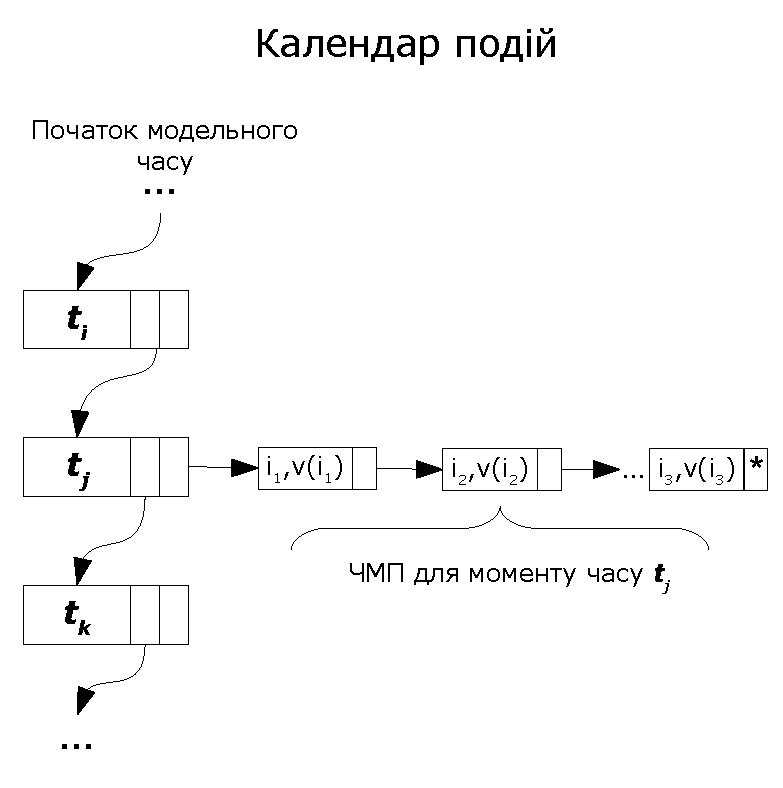
\includegraphics[width=0.75\textwidth]{events-calendar}
  \caption{Список подій}\label{feqCalendar}
\end{figure}

Тут кожному моменту часу відповідає свій список ЧМП. Моменту часу впорядковані і пов'язані списком. Занесення нової події з використанням цього способу вимагає пошуку потрібного моменту часу шляхом перегляду відповідних вказівників.

\subsection{Дослідження та апробації алгоритмів моделювання логічних схем}

Загальний вигляд алгоритмів моделювання логічних схем з використанням ЧМП можна записати так:\\
\textbf{Алгоритм логічного моделювання}
\small\begin{verbatim}
WHILE (черга подій не порожня)
{
  T=наступний в черзі момент часу (який має події);
  Обробка подій даного моменту часу;
}
\end{verbatim}\normalsize

Було оглянуто декілька різних типів алгоритмів. Серед них найкраще вписуються в умови BUMMEL такі:
\begin{itemize}
  \item подієвий двопрохідний;
  \item подієвий однопрохідний.
\end{itemize}

За своїми якісними характеристиками для першої апробації відібрано було „вдосконалений двопрохідний алгоритм“, наведений нижче.

\textbf{Вдосконалений двопрохідний алгоритм}
\small\begin{alltt}
Обробка подій даного моменту часу T()
\{
  АктивніЕлементи \(=\emptyset\) /* множина активних елементів */
  FOR кожної події \((i, v`_i)\), зв’язаної з T /* що має події на виходах */
  \{
    \(v(i) = v`_i\); /* переписування нового значення */
    IF \(v`_i \neq v(i)\) THEN
    FOR кожного елемента \(j\) -- наступника, елемента, що обробляється \(i\)
    \{
      Зміна значень входів \(j\); /* переписування з виходу \(i\)*/
      Поповнення множини АктивніЕлементи елементом \(j\);
    \}
  \}
  FOR кожного елемента \(j\in\) АктивніЕлементи
  \{
    \(v`_j\) = моделювання елемента \((j)\);
    IF \(v`_j \neq lsv(j)\) THEN
    \{
      Постановка події \(j, v`_j\) в ЧМП в момент часу \(T+d(j)\);
      \(lsv(j)=v`_j\)
    \}
  \}
\}
\end{alltt}\normalsize

У алгоритмі, представленому вище, заносяться в ЧМП тільки "істинні події", при яких відбувається зміна сигналу. Перевага двопрохідного алгоритму полягає в тому, що він дозволяє уникнути повторних обчислень (моделювання одного і того ж логічного елемента) у разі наявності кратних подій, коли на входах має місце зміна декількох сигналів.

\textbf{Результати апробації.} Сам алгоритм працює доволі добре, принаймі в межах проведених тестів. Було досягнуто успіху в поєднанні таких функцій, як: додавання елементів в схему, підключення елементів між собою, відключення елементів. Але так і не вдалось досягнути коректності роботи алгоритму при видаленні елементів зі схеми. Проблема полягає не лише в реалізації якоїсь окремої функції, а в реалізації алгоритму вцілому так щоб усі функції працювали злагоджено. Не знайдено задовільного способу пристосування алгоритму і за основу його \emph{не прийнято}.

\textbf{Видозмінений однопрохідний алгоритм}\\*
Хоча це і однопрохідний алгоритм, але розроблений він був на основі вище наведеного двопрохідного алгоритму. Головною ідейною відмінністю даного алгоритму є те, що в ЧМП реєструються не елементи, які викликають подію, а елементи яких подія стосується.

Такий підхід покликаний вирішити проблему з видаленням елементів, яка виникала в попередньому алгоритмі. Нижче подано метод \textbf{LogicCircuit::step()}, який і являє собою реалізацію видозміненого алгоритму.

\begin{lstlisting}[language=Java]
@Override public void step()
{
  while(!feq.isEmpty())
  {
    Map.Entry<Integer, HashMap<BasicElement, HashMap<String, Double>>> head =
      feq.remove();
    Integer currentDelay = head.getKey();
    System.out.println("Delay: " + currentDelay);
    // for each event (element) in the queue for the current delay
    for (Map.Entry<BasicElement, HashMap<String, Double>> entry
      : head.getValue().entrySet())
    {
      BasicElement bEl = entry.getKey();
      HashMap<String, Double> elSignals = entry.getValue();
      HashMap<String, Double> signalsToProcess = new HashMap<>();
      for(String port : bEl.getPorts())
      {
        Double val = elementPortValue.get(bEl).get(port);
        if(elementPortConnection.containsKey(bEl)
                && elementPortConnection.get(bEl).containsKey(port))
        {
          Connection conn = elementPortConnection.get(bEl).get(port);
          // connection existance check
          if (conn != null)
          {
            BasicElement connEl = (BasicElement) conn.getOther(bEl);
            val = (val + elementPortValue.get(connEl)
              .get(conn.getElementPort(connEl))) / 2;
          }
        }
        signalsToProcess.put(port, val);
      }
      signalsToProcess.putAll(elSignals);
      Map<String, Double> processedSignals = bEl.process(signalsToProcess);
      for(Map.Entry<String, Double> ps : processedSignals.entrySet())
      {
        String port = ps.getKey();
        Double val = ps.getValue();
        if(val.compareTo(elementPortValue.get(bEl).get(port)) != 0)
        {
          // change circuit value
          elementPortValue.get(bEl).put(port, val);
          if (elementPortConnection.containsKey(bEl)
                  && elementPortConnection.get(bEl).containsKey(port))
          {
            Connection conn = elementPortConnection.get(bEl).get(port);
            // connection existance check
            if (conn != null)
            {
              BasicElement connEl = (BasicElement) conn.getOther(bEl);
              // register connected elements in the FEQ
              // for the further processing
              feq.addEvent(bEl.getDelay(), connEl,
                conn.getElementPort(connEl), val);
            }
          }
        }
      }
    }
  }
}
\end{lstlisting}

При цьому, функції структурної взаємодії зі схемою є доволі прості, на відміну від двопрохідного алгоритму. При його реалізації ці функції включали частково логіку самої обробки схеми, яка була винесена в окремий приватний метод моделі логічної схеми (\lstinline$LogicCircuit$). При даному алгоритмі вони виглядають так як подано нижче.

\begin{lstlisting}
connectElements(Element firstElement, String firstElementPort,
 	            Element secondElement, String secondElementPort)
{
  if(super.connectElements(firstElement, firstElementPort,
       secondElement, secondElementPort))
  {
    BasicElement fbe = (BasicElement)firstElement;
    BasicElement sbe = (BasicElement)secondElement;

    feq.addEvent(sbe.getDelay(), fbe, firstElementPort,
      elementPortValue.get(sbe).get(secondElementPort));
    feq.addEvent(fbe.getDelay(), sbe, secondElementPort,
      elementPortValue.get(fbe).get(firstElementPort));

    return true;
  }
  return false;
}

disconnectElements(Element firstElement, String firstElementPort,
                   Element secondElement, String secondElementPort)
{
  BasicElement fbe = (BasicElement) firstElement;
  BasicElement sbe = (BasicElement) secondElement;

  feq.addEvent(0, fbe, firstElementPort, defaultValue());
  feq.addEvent(0, sbe, secondElementPort, defaultValue());

  super.disconnectElements(firstElement, firstElementPort,
    secondElement, secondElementPort);
}

addElement(Element element)
{
  super.addElement(element);

  Map<String, Double> elementSignals = new HashMap<>();
  for(String port : element.getPorts())
  {
    elementSignals.put(port, defaultValue());
  }
  elementPortValue.put(element, element.process(elementSignals));
}

removeElement(Element element)
{
  super.removeElement(element);
  elementPortValue.remove(element);
  return true;
}
\end{lstlisting}

\textbf{Результати апробації.} Проблема видалення елементів була вирішена цим алгоритмом. Але, як виявилось, реалізації цього алгоритм мали інший недолік - після певних ітерацій значення на входах/виходах елементів можуть бути некоректні. Внаслідок цього деякі схеми моделюються неправильно. Алгоритм \emph{не прийнято}.

Дослідження та апробації були проведені на розширеному наборі тестів, який використовувався при перевірці первинного алгоритму і набору елементів. В обох випадках отримано невдачу, але були досягнути наступні результати. Для більш реального моделювання, на відміну від, доволі описового, яке присутнє на даний момент в BUMMEL, було обрано реалізувати явні затримки елементів. В свою чергу, це потягнуло конкретизацію основи Моделі. Так як, в силу особливості задуму програми, цього потрібно уникати, було утворено окремий спеціалізований клас \lstinline$LogicCircuit$ для опрацювання затримок, власне, в якому і була реалізована \emph{Черга Майбутніх Подій}.

%\clearpage

%\section{Взаємодія з користувачем}

% відкопати старий код демонстрації властивостей на панелі

%1. Властивості елементів (панель налаштувань)\\
%2. Взаємодія з елементами/зі схемою (вікна налаштувань, натискання)

\clearpage

\section{Супутні архітектурні рішення в ході розробки}

\subsection{Інструменти для досліджень}

Спочатку розробка алгоритмів чи їх апробація проходила в стандартних умовах. Тобто новий алгоритм писався на місці старого, запускався і перевірявся на коректність. Також правився код в тестах для нового алгоритму. Після декількох таких перевірок стало зрозуміло, що потрібен якийсь інструмент, який автоматизує частину дослідження.

Так постала ідея порівняльного аналізу в режимі реального часу. Було використано \lstinline$@ServiceProvider$ та механізм \lstinline$Lookup$, які надає NetBeans Platform для одночасного підвантаження всіх наявних алгоритмів моделювання. Таким чином запуск тестів було видозмінено так, щоб вони запускали всі тести на усіх підвантажених в даний момент алгоритмах. В результаті, отримано таблиці порівнянь проходження тестів в різних алгоритмах.

Також ситуація була покращена і для користувача-дослідника. На основі механізму контекстно залежний подій (Context dependent \lstinline$@Action$) було розроблено динамічно генероване меню, що дає можливість відкрити одночасно декілька редакторів, які в основі використовуватимуть різні алгоритми. Тобто тепер користувач може в режимі реального часу випробовувати різні алгоритми одночасно.

\clearpage

\section{Охорона праці та безпеки в надзвичайних ситуаціях}

\subsection{Вступ}
З розвитком науково-технічного прогресу важливу роль грає можливість безпечного виконання людьми своїх трудових обов'язків.
Охорона здоров'я людей що працюють, забезпечення безпеки умов праці, ліквідація професійних захворювань і виробничого травматизму становить основу людської безпеки. Проте не варто забувати, що небезпечні чинники можуть діяти на людський організм не-поодинці, а взаємопов’язано. Але нажаль ми не можемо проаналізувати всі можливі комбінації сукупної дії небезпечних та шкідливих чинників. Невід’ємним елементом сьогодення є те, що людина проводить половину свого дня у приміщені за роботою.
Мета роботи – вивчення безпеки праці на робочому місці, вплив шкідливих чинників на працюючу особу й відчуття міри захисту від неї.
У зв’язку з цим була створена та розвивається наука про безпеку праці та життєдіяльності людини. Це комплекс заходів, вкладених у забезпечення безпеки людини у середовище проживання, збереження здоров'я, розробку методів і засобів захисту за методом зниження впливу шкідливих і найнебезпечніших чинників до допустимих значень, вироблення заходів для обмеження шкоди та ліквідацію наслідків надзвичайних ситуацій мирного й військової часу.
Під час виконання бакалаврської роботи було використано ряд різноманітного приладдя яке дає змогу опрацьовувати низку матеріалу, а саме комп’ютери, принтери, сканери. Не враховуючи приміщення в якому відбувається цей тривалий процес, а саме лабораторії, комп’ютерні класи
За умов роботи з ПК виникають наступні небезпечні та шкідливі чинники: несприятливі мікрокліматичні умови, освітлення, електромагнітні випромінювання, забруднення повітря шкідливими речовинами (джерелом яких може бути принтер, сканер), шум, вібрація, електричний струм, електростатичне поле, напруженість трудового процесу .


\subsection{Аналіз стану умов праці}
\subsubsection{Характеристика виробничого середовища та чинників трудового процесу}
\begin{itemize}
  \item Магістерська робота виконувалась і оформлювалась у центрі інформаційних технологій, який знаходиться у приміщенні ЛНУ ім. І. Франка в головному корпусі (вул. Університетська, 1).
  \item Приміщення розташовано на першому поверсі триповерхового будинку. У приміщенні розташовано 3 робочих місць з комп’ютерами. Розміри даного приміщень складають: довжина – 10 м, ширина – 6 м, висота – 3,5 м, тобто загальна фактична площа складає 60 м2.
  \item Необхідна площа на 3 робочих місця із установленими ПК складає 18 м2, що не перевищує фактичну. Обсяг кабінету на одного працюючого складає 70.м3, отже відповідає нормі (ДНАОП 0.00-1.31-99) [3] – не менше 20 м3. Площа одного робочого місця з відео дисплейним терміналом повинна бути не менше 6 м. кв, а об’єм не менше 20м.кб. Робочі місця розташовані від стіни з вікнами 1.5 м. а від бокових стін 1 м. Відстані між боковими поверхнями відео дисплеїв 1.2 м, а від тильного боку одного до екрану другого 2.5 м( я не знаю точно як порахувати на 10 робочих мість)(в цьому розділі  не наводьте нормативів, лише  те що реально  є. Це можна видалити)
  \item Загальна кількість робочих місць 10.
  \item Приміщення розташоване з північно-західною орієнтацією вікон. Мікроклімат у приміщенні забезпечує комфортне самопочуття людини. Оптимальна температура в приміщені становить: в теплий період року 23–25 °С, у холодний 22–24 °С. Відносна вологість повітря коливається в межах 60-40 \%. Швидкість руху повітря не перевищує 0.2 м/с – у теплий період часу, а у холодний 0.1 м/с. Приміщення з відеодисплейним терміналом оснащене припливно-витяжною вентиляцією та забезпечене природним вентилюванням.
  \item Освітлення приміщення змішане: природне і штучне. При цьому коефіцієнт природного освітлення не менше 1,5 \%, освітленість при штучному освітлені в площині робочої поверхні становить 300-500лК. Також допускається локальне освітлення з освітленістю екрана не більше 300 лК.
  \item У даному приміщені не має наявних хімічних речовин. Основним джерелом небезпек під час роботи з персональним комп’ютером є відеодисплейний термінал на основі електронно-променевої трубки. Більш безпечні відеодисплейні термінали з плазмовими та рідинно-кристалічними екранами. Крім безпосереднього впливу на організм людини, робота відеодисплейних терміналів має ще й опосередкований вплив, а саме: зумовлює порушення балансу аероіонів у зоні дихання користувача і призводить до зменшення кількості від’ємних аероіонів, які мають суттєвий вплив на імунну систему організму. Пониження імунітету людини внаслідок зменшення негативних аероіонів зумовлює інші порушення в організмі, зокрема й тих, що непов’язані з роботою на персональному комп’ютері.
  \item У приміщені наявна аптечка. 
  \item До засобів гасіння пожеж належать встановлені пожежні стволи, внутрішні пожежні водопроводи, вогнегасники, сухий пісок, азбестові ковдри. Пожежні крани встановлені в коридорах, на сходових клітках та вході. Приміщення забезпечені вогнегасниками. Для виявлення стадії загоряння та оповіщення використовують системи автоматичної пожежної сигналізації.
  \item На робочому місці викладачі проводять повний інструктаж з  охорони праці, повідомлять де розміщені плани будівлі, додаткові входи і виходи, розміщення вогнегасників. Також повідомлять про ряд небезпечних речовин та чинників, що впливають на наш організм.
\end{itemize}
\subsubsection{Опис трудового процесу} 
Негативний вплив на організм людини виникає через неадекватне (надто велике або надто мале) навантаження на окремі системи організму. Такі перекоси у напруженні різних систем організму, що трапляються підчас роботи з відеодисплейним терміналом, зокрема, значна напруженість зорового аналізатора і довготривале малорухоме положення перед екраном, не тільки не зменшують загального напруження, а навпаки, призводять до його посилення і прояву стресових реакцій.
Виконання бакалаврської роботи належить до легких робіт згідно класифікації робіт за ступенем важкості.
Основним робочим становищем є положення сидячи. Робоча поза сидячи викликає мінімальне стомлення людини. Раціональне планування робочого місця передбачає чіткий лад і сталість розміщення предметів. Те, що потрібно виконувати частіше, лежить у зоні легкої досяжності робочого простору. 
Можна вважати, що робоче місце досить добре пристосоване для ефективного виконання поставлених завдань і не приводить до погіршення продуктивності праці та погіршення самопочуття чи здоров’я.
\subsubsection{Аналіз методів дослідження, обладнання та характеристика речовин}
Під час виконання бакалаврської роботи. використовують персональні комп’ютери та периферійні пристрої (лазерні та струменеві друки, копіювальну техніку, сканери). Негативний вплив цих пристроїв на організм людини виникає через неадекватне (надто велике або надто мале) навантаження на окремі системи організму. Такі перекоси у напруженні різних систем організму, що трапляються під час роботи з ПК, зокрема, значна напруженість зорового аналізатора і довготривале малорухоме положення перед екраном, не тільки не зменшують загального напруження, а навпаки, призводять до його посилення і прояву стресових реакцій. Найбільшому ризику виникнення різноманітних порушень піддаються: органи зору, м’язово-скелетна система, нервово-психічна діяльність, репродуктивна функція у жінок.
Робота з комп’ютером характеризується значною розумовою напругою і нервово-емоційним навантаженням, високою напруженістю зорової праці та досить великим навантаженням на м’язи рук під час роботи з клавіатурою.
У процесі роботи з комп'ютером необхідно дотримуватися правильного режиму праці та відпочинку. Інакше у людини відзначаються значна емоційна напруга зорового апарату, що може призвести до появи головного білю, дратівливості, порушення сну, почуття виснаження. Раціональний режим праці та відпочинку передбачає запровадження регламентованих перерв, рівномірний розподіл навантаження протягом робочого дня, регулярні комплекси вправ для очей, рук, хребта для  поліпшення мозкового кругообігу та психофізіологічного розвантаження.
З метою запобігання перевантаження організму як в цілому, так і окремих його функціональних систем, передусім зорового та рухового аналізаторів, центральної нервової системи, загальний час щоденної роботи з відеодисплейним терміналом треба обмежити чотирма годинами та обов’язково дотримуватись регламентованих перерв.
Робота з ПК супроводжується також виділенням значної кількості тепла, шуму, вібрації та електромагнітних випромінювань.

\subsection{Організаційно-технічні заходи}
\subsubsection{Організація робочого місця і роботи}
Санітарно-гігієнічні та ергономічні вимоги до параметрів робочого місця, розміщення обладнання, пристроїв та персонального комп’ютера на ньому, психофізіологічні особливості праці (напруженість трудового процесу).
Робоче місце – це зона трудових дій працівника, обладнана для виконання певних операцій виробничого процесу, де взаємодіють три головні елементи праці – предмет, засоби і суб’єкт праці. На одному робочому місці можуть працювати два або кілька працівників, які виконують спільне завдання.  Наукова організація робочого місця передбачає створення працівникові всіх необхідних умов для високопродуктивної і високоякісної праці за можливо менших фізичних зусиль і мінімальному нервовому напруженні та передбачає:
\begin{itemize}
\item оснащеність робочого місця відповідним основним і допоміжним устаткуванням, технологічною і організаційною оснасткою;
\item раціональне планування, тобто найзручніше і найефективніше розміщення усіх елементів робочого місця для трудового процесу;
\item створення безпечних і здорових умов праці.
Просторова організація робочого місця повинна забезпечувати:
\item відповідність планування робочого місця санітарним і протипожежним нормам і вимогам;
\item безпеку працівникам;
\item відповідність просторових відношень між елементами робочого місця, антропометричними, біомеханічними, фізіологічними, психофізіологічними і психічними можливостями людини, що працює;
\item можливість виконання основних і допоміжних операцій в робочому положенні, що відповідає специфіці трудового процесу, в раціональній робочій позі і з використанням найбільш ефективних прийомів праці;
\item вільне переміщення працівника за оптимальними траєкторіями;
\item достатню площу для розміщення обладнання, інструменту, засобів контролю, деталей та ін.
Просторові та розмірні співвідношення між елементами робочого місця повинні дозволяти:
\item розміщення працівника з врахуванням робочих рухів і переміщень згідно з технологічним процесом;
\item оптимальний огляд джерела візуальної інформації;
\item зміну робочої пози і положення;
\item раціональне розміщення основних і допоміжних засобів праці.
\end{itemize}
Обов’язковою умовою є те, що на робочому місці повинні знаходитись лише ті технічні засоби, які необхідні для виконання робочого завдання, і розміщуватися вони повинні в межах досяжності з метою виключення частих нахилів і поворотів корпусу людини, що працює.
Під час роботи з персональним комп’ютером повинні бути дотримані наступні вимоги.
Вимоги до приміщення. Площу приміщень, в яких розташовують персональні комп’ютери, визначають згідно з чинними нормативними документами з розрахунку на одне робоче місце, обладнане ПК:
\begin{itemize}
\item площа — не менше 6,0 м2;
\item об’єм — не менше 20,0 м3, з урахуванням максимальної кількості осіб, які одночасно працюють у зміні;
\item робочі місця повинні бути розташовані на відстані не менше ніж 1 м від стіни з вікном;
\item відстань між бічними поверхнями комп’ютерів має бути не меншою за 1,2 м;
\item відстань між тильною поверхнею одного комп’ютера та екраном іншого не повинна бути меншою 2,5 м;
\end{itemize}
Прохід між рядами робочих місць має бути не меншим 1 м.
Користування ПК є основним видом діяльності, то ПК і його периферійні пристрої (принтер, сканер) розміщується на основному робочому столі, як правило, з лівого боку.
Вимоги до організації робочого місця з ПК. Конструкція робочого місця користувача ПК має забезпечувати підтримання оптимальної робочої пози з такими ергономічними характеристиками: 
\begin{itemize}
\item ступні ніг — на підлозі або на підставці для ніг; 
\item стегна — в горизонтальній площині; 
\item передпліччя — вертикально; 
\item лікті — під кутом 70–90° до вертикальної площини; 
\item зап’ястя зігнуті під кутом не більше 20° відносно горизонтальної площини; 
\item нахил голови — 15–20° відносно вертикальної площини.
\end{itemize}
Якщо користування ПК є основним видом діяльності, то ПК і його периферійні пристрої (принтер, сканер) розміщується на основному робочому столі, як правило, з лівого боку. Якщо використання ПК є періодичним, то він, як правило, розміщується на приставному столі, переважно з лівого боку від основного робочого столу.
Кут між поздовжніми осями основного та приставного столів має бути 90–140°.
Висота робочої поверхні столу для ПК має бути в межах 680–800 мм, а ширина — забезпечувати можливість виконання операцій в зоні досяжності моторного поля.
Рекомендовані розміри столу: висота 725 мм, ширина 600–1400 мм, глибина 800–1000 мм.
Робочий стіл для ПК повинен мати простір для ніг висотою не менше 600 мм, шириною не менше 500 мм, глибиною на рівні колін не менше 450 мм, на рівні витягнутої ноги — не менше 650 мм.
Робочий стіл для ПК, як правило, має бути обладнаним підставкою для ніг шириною не менше 300 мм та глибиною не менше 400 мм, з можливістю регулювання по висоті в межах 150 мм та кута нахилу опорної поверхні - в межах 20°. Підставка повинна мати рифлену поверхню та бортик на передньому краї заввишки 10 мм. Застосування підставки для ніг тими, у кого ноги не дістають до підлоги, є обов’язковим.
Робоче сидіння (сидіння, стілець, крісло) користувача ПК повинно мати такі основні елементи: сидіння, спинку, стаціонарні або знімні підлокітники. У конструкцію сидіння можуть бути введені додаткові елементи, що не є обов’язковими: підголовник та підставка для ніг. 
Робоче сидіння користувача ПК повинно бути підйомно-поворотним, таким, що регулюється за висотою, кутом нахилу сидіння та спинки, за відстанню спинки до переднього краю сидіння, висотою підлокітників. Регулювання кожного параметра має бути незалежним, плавним або ступінчатим, мати надійну фіксацію.
Хід ступінчатого регулювання елементів сидіння має становити для лінійних розмірів 15–20 мм, для кутових – 2–5°. Зусилля під час регулювання не повинні перевищувати 20 Н. Ширина та глибина сидіння повинні бути не меншими за 400 мм. Висота поверхні сидіння має регулюватися в межах 400–500 мм, а кут нахилу поверхні - від 15° вперед до 5° назад. Поверхня сидіння має бути плоскою, передній край - заокругленим. Висота спинки сидіння має становити 300±20 мм, ширина - не менше 380 мм, радіус кривизни в горизонтальній площині - 400 мм. Кут нахилу спинки повинен регулюватися в межах 0–30° відносно вертикального положення. Відстань від спинки до переднього краю сидіння повинна регулюватись у межах 260–400 мм.
Для зниження статичного напруження м’язів рук необхідно застосовувати стаціонарні або знімні підлокітники довжиною не менше 250 мм, шириною 50–70 мм, що регулюються по висоті над сидінням у межах 230±30 мм та по відстані між підлокітниками в межах 350–500 мм.
Поверхня сидіння, спинки та підлокітників має бути напівм’якою, з неслизьким, ненаелектризовувальним, повітронепроникним покриттям та забезпечувати можливість чищення від бруду.
Монітор та клавіатура мають розташовуватися на оптимальній відстані від очей користувача, але не ближче 600 мм, з урахуванням розміру алфавітно-цифрових знаків та символів.
Розташування монітору має забезпечувати зручність зорового спостереження у вертикальній площині під кутом ±30° від лінії зору працівника.
Клавіатуру слід розміщувати на поверхні столу або на спеціальній, регульованій за висотою, робочій поверхні окремо від столу на відстані 100–300 мм від краю, ближчого до працівника. Кут нахилу клавіатури має бути в межах 5–15°.
Розміщення принтера або іншого пристрою введення-виведення інформації на робочому місці має забезпечувати добру видимість монітору, зручність ручного керування пристроєм введення-виведення інформації в зоні досяжності моторного поля: по висоті 900–1300 мм, по глибині 400–500 мм.
При потребі високої концентрації уваги під час виконання робіт з високим рівнем напруженості суміжні робочі місця з ПК необхідно відділяти одне від одного перегородками висотою 1,5–2 м.
Режим праці та відпочинку користувачів ПК встановлюють з урахуванням психофізіологічної напруженості їхньої праці, динаміки функціонального стану систем організму та працездатності. Раціональний режим праці та відпочинку передбачає запровадження регламентованих перерв, рівномірний розподіл навантажень протягом робочого дня, регулярні комплекси вправ для очей, рук, хребта, поліпшення мозкового кругообігу та психофізіологічне розвантаження.
З метою запобігання перевантаження організму як в цілому, так і окремих його функціональних систем, передусім зорового та рухового аналізаторів, центральної нервової системи, загальний час щоденної роботи з ПК обмежують. Робота з персональним комп’ютером вважається основною, якщо вона займає не менше як 50 % часу робочого дня чи робочої зміни.
З урахуванням характеру трудової діяльності, напруженості та важкості праці з використанням ПК під час основної роботи за восьмигодинної робочої зміни встановлюють додаткові регламентовані перерви:
\begin{itemize}
\item для розробників програм тривалістю 15 хв через кожну годину роботи;
\item для операторів персональних комп’ютерів тривалістю 15 хв через дві години роботи;
\item для операторів комп’ютерного набору тривалістю 10 хв через кожну годину роботи.
\end{itemize}
За жодних умов безперервна робота з ПК не повинна перевищувати чотири години.
За дванадцятигодинної робочої зміни протягом перших восьми годин регламентовані перерви встановлюють аналогічно до восьмигодинної робочої зміни, а протягом останніх чотирьох годин тривалістю 15 хв через кожну годину незалежно від характеру трудової діяльності.

Навчання та інструктажі з безпеки праці. Перед допуском до самостійної роботи кожен працівник має право на навчання з питань охорони праці і роботодавець зобов’язаний провести таке навчання у вигляді двох інструктажів з питань охорони праці:
\begin{itemize}
\item вступного, який проводять працівники служби охорони праці об’єкта господарювання з усіма працівниками, яких приймають на роботу незалежно від їхньої освіти та стажу роботи за програмою, в якій подають загальні питання охорони праці із врахуванням її особливостей на об’єкті господарювання;
\item первинного, який проводять керівники структурних підрозділів на робочому місці з кожним працівником до початку їхньої роботи на цьому робочому місці.
\end{itemize}
Проходження цих інструктажів з питань охорони праці підтверджується записами у відповідних журналах обліку інструктажів і скріплюється підписами осіб, які проводили інструктажі та осіб, які отримали інструктажі.
Організаційні заходи перед початком, під час і після завершення роботи.
Працівники до початку роботи повинні перевірити візуально наявність і справність електрообладнання та його заземлення, а під час виконання роботи не залишати без нагляду обладнання, яке використовують. Після закінчення роботи необхідно прибрати робоче місце, відключити всі електроприлади від електромережі, перекрити крани водо- та газомережі.

\subsubsection{Санітарно-гігієнічні вимоги до умов праці}
Санітарно-гігієнічні вимоги до умов праці під час виконання роботи описують:
Нормативи з параметрів мікроклімату, освітлення приміщень, рівнів шуму, вібрації та електромагнітних випромінювань.
Мікроклімат виробничих приміщень характеризують температурою, вологістю та  швидкістю руху повітря, а також інтенсивністю радіації, переважно в інфрачервоній та ультрафіолетовій областях спектру електромагнітних випромінювань.
Параметри мікроклімату у приміщеннях повинні забезпечувати комфортне самопочуття організму. Тому у виробничих приміщеннях повинна бути надійна система кліматичного контролю. 
Параметри мікроклімату закритих приміщень нормують санітарні норми ДСН 3.3.6.042‑99. Оптимальні параметри мікроклімату закритих приміщень наведені в таблиці.
Оптимальні параметри мікроклімату закритих приміщень
Категорія
робіт	Температура, ºС	Відносна вологість повітря, %	Швидкість руху повітря, м/с			
холодний період року	теплий період року	холодний період року	теплий період року	холодний період року	теплий період року
Іа	22–24	23–25	60–40	60–40	0,1	0,1
Іб	21–23	22–24	60–40	60–40	0,1	0,2
Освітлення приміщень та робочих місць. Ще один важливий чинник, від якого залежать працездатність і здоров’я людини, – це освітлення. Світло регулює всі функції людського організму і впливає на психологічний стан і настрій, обмін речовин, гормональний фон і розумову активність. 
Найздоровіше освітлення забезпечує природне світло. Його ефективне використання можливе, якщо глибина приміщень не перевищує 6 м. Окрім того, хорошим вирішенням можуть будуть скляні перегородки, що забезпечують зорову і звукову ізоляцію, але в той же час не перешкоджають проникненню природного світла. 
Відносно вікон робоче місце повинно бути розміщено так, щоб природне світло було збоку, переважно з лівого та забезпечувати коефіцієнт природної освітленості не нижче 1,5 \%. Освітленість за штучного освітлення в площині робочої поверхні має становити 300–500 Лк. Якщо таких значень освітленості досягнути не можна, то допускається локальне освітлення, при цьому освітленість екрана не може перевищувати 300 Лк. Відношення яскравості робочих поверхонь не повинно бути більшим ніж 3:1, а яскравості робочих поверхонь і стін (іншого обладнання) - 5:1. Робоче місце, обладнане ПК повинно бути розташоване так, щоб уникнути попадання в очі прямого світла.
Щоб уникнути світлових відблисків від екрану та клавіатури необхідно використовувати комп’ютерне обладнання з матовою поверхнею. Для захисту очей від прямого сонячного світла чи джерел штучного освітлення необхідно застосовувати захисні козирки та жалюзі на вікнах. 
Вимоги до рівнів шуму та вібрації. Шум часто є причиною зниження рівня працездатності, підвищення рівня загальної та професійної захворюваності, частоти виробничих травм. Шум як стрес-чинник є загальнобіологічним подразником, який негативно впливає на всі органи і системи організму. У разі тривалого систематичного впливу шуму може виникнути патологія з переважним ураженням слуху, центральної нервової і серцево-судинної систем.
Гігієнічне нормування рівнів шуму. Допустимі рівні звукового тиску у октавних смугах частот, еквівалентні рівні звуку на робочих місцях встановлені санітарними нормами виробничого шуму, ультразвуку та інфразвуку ДСН 3.3.6.037-99, і для творчої та наукової роботи, навчання, не повинні перевищувати 50 дБА. 
Вібрація приводить тіло і його структурні частини в коливний рух. Розрізняють поперечні, поздовжні і крутильні коливання. За впливом на людину вібрації ділять на місцеві і загальні. Загальні вібрації викликають коливання тіла людини, місцеві – лише окремі частини тіла. Тривала дія вібрацій на організм людини призводить до порушень в центральній нервовій та серцево-судинній системах, погіршує загальний стан людини – появляються втома, головний біль тощо.
Колективні  та індивідуальні засоби і заходи захисту від шкідливого впливу виробничих чинників на здоров’я людини .
Облаштовуючи приміщення для роботи з ПК, потрібно передбачити припливно-витяжну вентиляцію або кондиціювання повітря. Надходження свіжого повітря регулюють, виходячи із таких умов (вказаний об’єм приміщення припадає на одне робоче місце з ПК):
\begin{itemize}
\item	якщо об’єм приміщення 20 м3, то потрібно подати не менш як 30 м3/год повітря;
\item	якщо об’єм приміщення у межах від 20 до 40 м3, то потрібно подати не менш як 20 м3/год повітря;
\item	якщо об’єм приміщення становить понад 40 м3, допускається природна вентиляція, у випадку, коли немає виділення шкідливих речовин.
\end{itemize}
Захист від шуму та вібрацій. Усунення шуму в приміщенні є однією з найскладніших проблем, оскільки джерела шуму різноманітні й потребують комплексу заходів технічного, організаційного і медичного характеру на всіх стадіях проектування, будівництва, експлуатації машин і устаткування. Відомі три головні напрямки зменшення впливу шуму на організм людини:
\begin{itemize}
\item	зменшення рівня шуму у джерелі виникнення, застосування раціональних конструкцій, нових матеріалів і технологічних процесів;
\item	звукоізоляція устаткування за допомогою глушників, резонаторів, кожухів, захисних конструкцій, оздоблення стін, стелі, підлоги тощо;
\item	використання засобів індивідуального захисту.
\end{itemize}
Заходи особистої гігієни на робочому місці (підтримання чистоти, миття лабораторного посуду, рук тощо).
Заходи особистої гігієни на робочому місці передбачають щоденне вологе прибирання, утримання у чистоті робочого місця, наявність на робочому місці тільки необхідних для роботи засобів. На робочому місці необхідно дотримуватись вимог правил внутрішнього розпорядку, зокрема, заборонено приймати їжу, пити, курити та ін.

\subsubsection{Заходи щодо безпеки під час виконання бакалаврської роботи}
1.	Заходи безпеки під час експлуатації персонального комп’ютера та периферійних пристроїв передбачають:
\begin{itemize}
\item	правильну організацію робочого місця та дотримання оптимальних режимів праці та відпочинку під час роботи з ПК;
\item	експлуатацію сертифікованого обладнання;
\item	дотримання заходів електробезпеки;
\item	забезпечення оптимальних параметрів мікроклімату;
\item	забезпечення  раціонального освітлення робочого місця;
\item	зниження рівня шуму та вібрації.
\end{itemize}
2.	Заходи безпеки під час експлуатації інших електричних приладів передбачають дотримання таких правил:
\begin{itemize}
\item	постійно стежити за справним станом електромережі, розподільних щитків, вимикачів, штепсельних розеток, лампових патронів, а також мережевих кабелів живлення, за допомогою яких електроприлади під’єднують до електромережі;
\item	постійно  стежити за справністю ізоляції електромережі та мережевих кабелів, не допускаючи їхньої експлуатації з пошкодженою ізоляцією;
\item	не тягнути за мережевий кабель, щоб витягти вилку з розетки;
\item	не закривати меблями, різноманітним інвентарем вимикачі, штепсельні розетки; 
\item	не підключати одночасно декілька потужних електропристроїв до однієї розетки, що може викликати надмірне нагрівання провідників, руйнування їхньої ізоляції, розплавлення і загоряння полімерних матеріалів;
\item	не залишати включені електроприлади без нагляду; 
\item	не допускати потрапляння всередину електроприладів крізь вентиляційні отвори  рідин або металевих предметів, а також не закривати їх та підтримувати в належній чистоті, щоб уникнути перегрівання та займання приладу;
\item	не ставити на електроприлади матеріали, які можуть під дією теплоти, що виділяється, загорітися (канцелярські товари, сувенірну продукцію).
\end{itemize}
\subsection{Безпека в надзвичайних ситуаціях}
\subsubsection{Протипожежні та противибухові заходи}
Пожежа - це неконтрольоване горіння, яке супроводжується виділенням тепла, світла, диму та інших продуктів. Горіння виникає за таких трьох умов: наявності окисника, наявності горючої речовини, наявності температури, за якої горюча речовина може самостійно горіти. Якщо немає хоча б однієї із цих умов, горіння стає неможливим. На цьому постулаті ґрунтується переважна більшість профілактичних заходів, спрямованих на відвернення пожеж.
У приміщенні в якому виконувалась бакалаврська робота не використовують пожежовибухонебезпечні речовини і матеріали. Найбільш ймовірним джерелом пожеж може бути несправність електрообладнання та загорянням горючих матеріалів, зокрема, канцелярського приладдя, паперу.
1.	Можливі причини виникнення пожежі та вибухів на робочому місці.
Головними причинами виникнення пожеж та вибухів є:
\begin{itemize}
\item	порушення пожежних норм і правил;
\item	порушення правил встановлення та експлуатації систем енергопостачання, опалення, вентиляції;
\item	порушення правил експлуатації електричного та газового обладнання;
\item	порушення правил зберігання пожежовибухонебез-печних матеріалів;
\item	використання відкритого вогню в заборонених місцях;
\item	погане знання персоналом протипожежних правил;
\item	необережна поведінка з вогнем.
\end{itemize}
2.	Заходи запобігання виникненню пожежі та вибуху, первинні засоби пожежогасіння.
Переважна більшість пожеж починається із невеличкого вогнища. Тому його своєчасну ліквідацію розглядаємо як профілактичний захід щодо недопущення його розширення до масштабів пожежі. Ліквідувати вогнище можна, усунувши одну із трьох умов виникнення горіння. Видалити горючу речовину із вогнища не завжди можна, а припинити доступ кисню до неї або/і понизити її температуру можна завжди, якщо своєчасно використати первинні засоби гасіння пожеж: воду, пісок або вогнегасники.
Вода – універсальний засіб для гасіння пожеж, оскільки її застосування завдяки випаровуванню дає змогу як понизити температуру горючої речовини, так і зменшити доступ кисню до неї. Проте нею не можна гасити електроустановки під напругою та легкозаймисті рідини. Для цього треба використовувати пісок, хоча він є менш ефективним.
Вогнегасники, залежно від природи вогнегасної речовини бувають різних типів. Найпоширеніші з них:
\begin{itemize}
\item	хімічно-пінні (ВХП–10);
\item	повітряно-пінні  (ВПП–5, ВПП–10);
\item	вуглекислотні (ВВ–2, ВВ–3, ВВ–5);
\item	порошкові (ВП–2–01, ВП–2Б, ВПУ–2, ВП–5–01, ВП–8Б).
\end{itemize}
Важливо пам’ятати, що хімічно-пінними та повітряно-пінними вогнегасниками не можна гасити електрообладнання під напругою. Потрібно своєчасно і вміло використовувати вогнегасники для локалізації невеликих ділянок горіння, оскільки час їхньої дії є досить малий, у найкращому випадку - до 60 с.
Також варто зазначити, що користуючись газовими приладами необхідно дотримуватись таких вимог:
\begin{itemize}
\item	забезпечити надійне вентилювання приміщення (відкрийте кватирки вікон, не закривайте отвори та решітки вентиляційних каналів, забезпечте постійне провітрювання приміщення);
\item	перевірити наявність тяги у димоході (за відсутності чи слабій тязі не користуйтесь газовими приладами – це смертельно небезпечно!);
\item	не встановлювати в приміщенні, де є газові прилади з відведенням продуктів згоряння у димові канали, витяжну механічну систему вентилювання;
\item	не користуватися газовими приладами за несправної автоматики безпеки;
\item	не залишати без нагляду газові прилади у робочому стані;
\item	не використовувати приміщення, де встановлено газові прилади, для сну та відпочинку;
\item	не використовувати газові плити для обігріву приміщення;
\item	перекривати крани після користування газовими приладами.
\end{itemize}

\subsubsection{Організація евакуації працівників}
Виконуючи бакалаврську роботу було проаналізовано схему шляхів евакуації, які забезпечують якнайшвидше і найбезпечніше виведення людей з небезпечних зон.
Проведення організованої евакуації з виробничих та інших приміщень і будівель, запобігання проявам паніки і недопущення загибелі людей забезпечують шляхом складання плану евакуації з розробленням схеми евакуаційних шляхів та виходів. На підприємстві має бути встановлено порядок оповіщення людей про пожежу, з яким необхідно ознайомити всіх працівників. 
Серед загальних вимог до евакуаційних шляхів та виходів необхідно відмітити, що ними можуть бути дверні отвори, якщо вони ведуть з приміщень: 
\begin{itemize}
\item	безпосередньо назовні; 
\item	на сходовий майданчик з виходом назовні безпосередньо або через вестибюль; 
\item	у прохід або коридор з безпосереднім виходом назовні або на сходовий майданчик; 
\item	у сусідні приміщення того ж поверху, що не містять виробництв, які належать за вибухопожежною та пожежною небезпекою до категорій А, Б і В та мають безпосередній вихід назовні або на сходовий майданчик. 
\end{itemize}
Для безпечної евакуації шляхи та виходи мають відповідати таким вимогам: 
\begin{itemize}
\item	евакуаційні шляхи і виходи повинні утримуватися вільними, не захаращуватися та у разі потреби забезпечувати евакуацію всіх людей, які перебувають у приміщеннях;
\item	кількість та розміри евакуаційних виходів, їхні конструктивні рішення, умови освітленості, забезпечення незадимленості, протяжність шляхів евакуації, їхнє оздоблення повинні відповідати протипожежним вимогам будівельних норм;
\item	у приміщенні, яке має один евакуаційний вихід, дозволяється одночасно розміщувати не більше 50 осіб, а у разі перебування в ньому понад 50 осіб повинно бути щонайменше два виходи, які відповідають вимогам будівельних норм;
\item	двері на шляхах евакуації повинні відчинятися в напрямку виходу з будівель (приміщень) і замикатися лише на внутрішні запори, які легко відмикаються.
\end{itemize}

\subsection{Висновки}
Згідно із проведеним аналізом можна побачити, що санітарно-гігієнічні та ергономічні умови праці відповідають нормативам і їх не треба покращувати. 

\clearpage
 
\section{Висновки}

Проведено аналіз архітектури електронної лабораторії BUMMEL. Особливістю даної програми є те, що найнижчий рівень Моделі (MVC) орієнтований на універсальну роботу з мережами. Тобто в межах розроблених інтерфейсів можна, конкретизуючи алгоритм в предметну область, додавши ті чи інші, необхідні для його коректної роботи, обмеження („звузивши“ інтерфейс збільшенням специфічних методів) моделювати не лише логічні чи фізичні схеми, а й багато інших процесів. Дана особливість накладає на процес розробки основи строге обмеження - уникати конкретизації.

Було виявлено, що програма містить деякі порушення архітектури MVC. В ході даної роботи було окреслено місця цих порушень, та представлено детальну структуру класів в UML діаграмах, де ці недоліки краще видно. Використавши цей матеріал було укладено набір інтерфейсів для подачі та можливості зміни властивостей, а також для взаємодії з досліджуваними об’єктами (гілка розробки \lstinline$VLEditor$).

Для допомоги у виконанні завдання виправлення моделювання логіки залучено патерни програмування \emph{Lookup} та \emph{Service Provider Interface} та розроблено механізм динамічного підвантаження наявних алгоритмів моделювання, їх тестування та подачу користувачу (як пункти меню для відкривання редакторів). На цьому етапі в класах \lstinline$ProjectModel$ (\textbf{M}VC) та \lstinline$EditorTopComponent$ (MV\textbf{C}) була реалізована можливість використовувати різні алгоритми, як нащадки \lstinline$Circuit$ (\textbf{M}VC).

Cтворені інструменти для спрощення досліджень алгоритмів моделювання процесів на графах сприяли дослідженню та спробам адаптації алгоритмів моделювання логічних схем. В роботі було оглянуто ряд різних алгоритмів логічного моделювання: компілятивних та інтерпретативних, наскрізних та подієвих. Найкраще в архітектуру програми і в межі інструментів розробки (Java, NetBeans Platform) вписуються одно- та двопрохідні подієві алгоритми.

В межах цієї роботи було проведено спробу пристосування вдосконаленого двопрохідного та самостійно розробленого (на основі попереднього) однопрохідного алгоритмів моделювання логічних схем. В обох випадках отримано невдачу, але були досягнути наступні результати. Для більш реального моделювання, на відміну від, доволі описового, яке присутнє на даний момент в BUMMEL, було обрано реалізувати явні затримки елементів. В свою чергу, це потягнуло конкретизацію основи Моделі. Так як, в силу особливості задуму програми, цього потрібно уникати, було утворено окремий спеціалізований клас \lstinline$LogicCircuit$ для опрацювання затримок, власне, в якому і була реалізована \emph{Черга Майбутніх Подій}.

Перед апробацією вищезазначених методів було проведено роботу по більш глибокому вивченню предметної області, розглянуто класифікацію алгоритмів моделювання. На основі отриманих даних можна окреслити наступні кроки подальшого розвитку програми:
\begin{itemize}
  \item завершення розробки спеціалізованих класів моделювання логіки;
  \item зведення спеціалізованих класів до універсальних шляхом моделювання процесів на глибшому рівні;
  \item реалізація інтерфейсу користувача через інтерфейси для взаємодії;
  \item випробування програми в межах університетського курсу -- в реальних умовах.
\end{itemize}

Приємно зазначити, що за рік цієї роботи BUMMEL було представлено на двох конференціях:
\begin{itemize}
  \item „Сучасні проблеми прикладної математики та інформатики“ \cite{thesis-MPoAMaCS};
  \item "FOSS Lviv 2013" \cite{thesis-foss2013}.
\end{itemize}
Можливо, це допоможе залученню до проекту сторонніх розробників вільного програмного забезпечення чи наукових лиць, зацікавлених даною тематикою.

Частково це вже відбулось, так як на конференціях поступало декілька пропозицій, які цікаві на сьогоднішній день і можуть бути реалізовані з деякою зміною даного функціоналу.

Приносить радість те, що над проектом працює жвава команда розробників, які привносять кожен щось своє і нове в даний продукт, діляться цікавими конструктивними ідеями та демонструють практичні рішення до різних проблем, що постають на шляху розвитку електронної лабораторії BUMMEL.

\clearpage

\section{Рекомендації}

Проведена робота привела до наступних висновків та ідей. Синтаксис мови Java є доволі громіздкий, а це ускладнює розробку чи апробацію алгоритмів та архітектурних елементів. На даному проекті, але в іншій роботі проводиться експеримент з переведенням частини програми на функціональну мову програмування Scala. Дане дослідження підтверджує актуальність таких експериментів і пошуку зручнішого синтаксису. Крім того, Java - компілятивна мова програмування і в межах даного проекту, який є доволі великий, багато часу іде на сам процес компіляції. Тому постає питання спроби використання інтерпретативних мов, де б можна було зразу ж подивитись результати експерименту. Це дуже зручно, особливо з точки зору досліджень.

Тестування та апробація алгоритмів моделювання логічного рівня показала, що поєднати ідею універсальної бази для моделювання процесів на мережах, графах і т.д. доволі складно. В кожному з випадків процес затримувався в певному місці, без видимого шляху доведення експерименту до працюючого результату. Для вирішення проблеми моделювання потрібно продовжити дослідження та підключити до співпраці людей з глибоким розумінням предметної області, так як інколи потрібно одночасно і широко та здалеку оглядати проблему, і пам’ятати про дрібниці в глибині моделювання.

Є ще один цікавий напрямок розвитку проекту. Думка та ідея про нього з’явилась внаслідок співпраці з Тимчуком Ю.А. та ознайомленням з його магістерською роботою \cite{thesis-Tymchuk}. Юрій запропонував створити зручний графічний редактор мережевих процесів на основі BUMMEL. Ця пропозиція наштовхнула мене на думку перевести BUMMEL з електронної лабораторії в платформу для досліджень моделювання різних процесів, або побудувати таку на базі цієї програми.

\clearpage

\addcontentsline{toc}{section}{Список використаних джерел}
\begin{thebibliography}{9}

%  \bibitem{alias}<АВТОР> \emph{<КНИГА>}
%     - <МІСЦЕ ВИДАННЯ> : <ВИДАВНИЦТВО>, <РІК>. - <К-КІСТЬ СТОРІНОК> с.

%  \bibitem{alias2}<АВТОР> \emph{<НАЗВА>}
%    [Електронний ресурс], <РІК>. Режим доступу:
%    \url{https://github.com/Uko/thesis-template}

  \bibitem{nb-6.9-dev-guide}Jürgen Petri \emph{NetBeans Platform 6.9 Developer's Guide}
     - Birmingham : Packt Publishing, 2010. - 275 с.

  \bibitem{nb-7-dev-guide}Heiko Böck \emph{The Definitive Guide to NetBeans Platform 7}
     - New York : APRESS, 2012. - 562 с.

  \bibitem{nb-7-cook}Rhawi Dantas \emph{NetBeans IDE 7 Cookbook}
     - Birmingham : Packt Publishing, 2011. - 308 с.

  \bibitem{thesis-MPoAMaCS}Тимчук Ю.А. \emph{Особливості організації робочого потоку при програмуванні симулятора BUMMEL}
    / Рикалюк Р.Є., Тимчук Ю.А., Михалевич І.А.
    // XVІІI Всеукраїнська наукова конференція „Сучасні проблеми прикладної математики та інформатики“
    - Львів : ЛНУ ім. І. Франка, 4-5 жовтня, 2012.

  \bibitem{thesis-foss2013}Михалевич І.А. \emph{Моделювання логічних елементів за допомогою симулятора логічних схем BUMMEL}
    / Рикалюк Р.Є., Тимчук Ю.А., Михалевич І.А.
    // Міжнародна конференція "FOSS Lviv 2013" Вільне програмне забезпечення та його використання в освіті, науці та бізнесі
    - Львів : ЛНУ ім. І. Франка, 18-21 квітня, 2013.

  \bibitem{intuit-modelling}\emph{Моделирование, тестирование и диагностика цифровых устройств}
    [Електронний ресурс], 2012. Режим доступу:
    \url{http://www.intuit.ru/studies/courses/3440/682/info}

  \bibitem{bib-logModNTest}\emph{Логическое моделирование и тестировании цифровых устройств}
     - Донецьк : ІПММ НАНУ, 2005. - 436 с.

  \bibitem{book-dltas}\emph{Digital logic testing and simulation}
     - John Wiley\&Sons, 2003. - 673 с.

  \bibitem{book-dstatd}\emph{Digital System Testing and Testable Design}
     - New York: Computer Science Press, 1990. – 652 с.

  \bibitem{book-potes}\emph{Principles of testing electronic systems}
     - John Wiley\&Sons, 2000. - 420 с.

  \bibitem{book-cdic}\emph{CMOS digital integrated circuits}
    Analysis and design - Boston: McGrow-Hill, 1999.

  \bibitem{book-ddmat}\emph{Моделирование и тестирование дискретных устройств}
     - Київ: Наукова думка, 1992. - 288 с.

  \bibitem{thesis-Tymchuk}Тимчук Ю.А. \emph{Розширення функціональності моделі FAMIX для побудови
абстрактних дерев коду Java- та Smalltalk-програм}
    [Електронний ресурс], 2013. Режим доступу:
    \url{http://uko.github.io/metamodels-thesis/thesis.pdf}

  \bibitem{book-eoetfdmamvc}\emph{Essentials of electronic testing for digital, memory and mixed-signal VLSI circuits}
    Kluwer academic publishers, 2001. - 690 с.

  \bibitem{book-solcwvlu}\emph{Синтез логических схем с использованием языка VHDL}
     - Москва: СОЛОН-Рб, 2002. - 384 с.

  \bibitem{book-apodd}\emph{Автоматизированное проектирование цифровых устройств}
     - Москва: Радио и связь, 1981. - 240 с.

  \bibitem{book-pblc}\emph{Pseudo-boolean logic circuits}
    IEEE Trans. On Comput. - 1986. - C.35, N7. - P.602-612

  \bibitem{book-tdb}\emph{Основы технической диагностики}
     - Москва: Энергия, 1976.- 464 с.

  \bibitem{book-CADMct}\emph{Тестирование КМОП-схем}
    Автоматика и телемеханика. - 1991. - №2. - с.3-34

  \bibitem{book-dlsiattep2pfs}\emph{Digital logic simulation in a timed-based, table-driven environment. Part 2. Parallel Fault Simulation}
    Computer, IEEE Comp. Society. - 1975. - N3. - P.38-49

\end{thebibliography}

\end{document}
